% Options for packages loaded elsewhere
% Options for packages loaded elsewhere
\PassOptionsToPackage{unicode}{hyperref}
\PassOptionsToPackage{hyphens}{url}
\PassOptionsToPackage{dvipsnames,svgnames,x11names}{xcolor}
%
\documentclass[
  12pt,
  a4paper,
  openany]{scrbook}
\usepackage{xcolor}
\usepackage[left=3cm,right=2.5cm,top=3cm,bottom=3cm]{geometry}
\usepackage{amsmath,amssymb}
\setcounter{secnumdepth}{2}
\usepackage{iftex}
\ifPDFTeX
  \usepackage[T1]{fontenc}
  \usepackage[utf8]{inputenc}
  \usepackage{textcomp} % provide euro and other symbols
\else % if luatex or xetex
  \usepackage{unicode-math} % this also loads fontspec
  \defaultfontfeatures{Scale=MatchLowercase}
  \defaultfontfeatures[\rmfamily]{Ligatures=TeX,Scale=1}
\fi
\usepackage{lmodern}
\ifPDFTeX\else
  % xetex/luatex font selection
\fi
% Use upquote if available, for straight quotes in verbatim environments
\IfFileExists{upquote.sty}{\usepackage{upquote}}{}
\IfFileExists{microtype.sty}{% use microtype if available
  \usepackage[]{microtype}
  \UseMicrotypeSet[protrusion]{basicmath} % disable protrusion for tt fonts
}{}
\makeatletter
\@ifundefined{KOMAClassName}{% if non-KOMA class
  \IfFileExists{parskip.sty}{%
    \usepackage{parskip}
  }{% else
    \setlength{\parindent}{0pt}
    \setlength{\parskip}{6pt plus 2pt minus 1pt}}
}{% if KOMA class
  \KOMAoptions{parskip=half}}
\makeatother
% Make \paragraph and \subparagraph free-standing
\makeatletter
\ifx\paragraph\undefined\else
  \let\oldparagraph\paragraph
  \renewcommand{\paragraph}{
    \@ifstar
      \xxxParagraphStar
      \xxxParagraphNoStar
  }
  \newcommand{\xxxParagraphStar}[1]{\oldparagraph*{#1}\mbox{}}
  \newcommand{\xxxParagraphNoStar}[1]{\oldparagraph{#1}\mbox{}}
\fi
\ifx\subparagraph\undefined\else
  \let\oldsubparagraph\subparagraph
  \renewcommand{\subparagraph}{
    \@ifstar
      \xxxSubParagraphStar
      \xxxSubParagraphNoStar
  }
  \newcommand{\xxxSubParagraphStar}[1]{\oldsubparagraph*{#1}\mbox{}}
  \newcommand{\xxxSubParagraphNoStar}[1]{\oldsubparagraph{#1}\mbox{}}
\fi
\makeatother


\usepackage{longtable,booktabs,array}
\usepackage{calc} % for calculating minipage widths
% Correct order of tables after \paragraph or \subparagraph
\usepackage{etoolbox}
\makeatletter
\patchcmd\longtable{\par}{\if@noskipsec\mbox{}\fi\par}{}{}
\makeatother
% Allow footnotes in longtable head/foot
\IfFileExists{footnotehyper.sty}{\usepackage{footnotehyper}}{\usepackage{footnote}}
\makesavenoteenv{longtable}
\usepackage{graphicx}
\makeatletter
\newsavebox\pandoc@box
\newcommand*\pandocbounded[1]{% scales image to fit in text height/width
  \sbox\pandoc@box{#1}%
  \Gscale@div\@tempa{\textheight}{\dimexpr\ht\pandoc@box+\dp\pandoc@box\relax}%
  \Gscale@div\@tempb{\linewidth}{\wd\pandoc@box}%
  \ifdim\@tempb\p@<\@tempa\p@\let\@tempa\@tempb\fi% select the smaller of both
  \ifdim\@tempa\p@<\p@\scalebox{\@tempa}{\usebox\pandoc@box}%
  \else\usebox{\pandoc@box}%
  \fi%
}
% Set default figure placement to htbp
\def\fps@figure{htbp}
\makeatother


% definitions for citeproc citations
\NewDocumentCommand\citeproctext{}{}
\NewDocumentCommand\citeproc{mm}{%
  \begingroup\def\citeproctext{#2}\cite{#1}\endgroup}
\makeatletter
 % allow citations to break across lines
 \let\@cite@ofmt\@firstofone
 % avoid brackets around text for \cite:
 \def\@biblabel#1{}
 \def\@cite#1#2{{#1\if@tempswa , #2\fi}}
\makeatother
\newlength{\cslhangindent}
\setlength{\cslhangindent}{1.5em}
\newlength{\csllabelwidth}
\setlength{\csllabelwidth}{3em}
\newenvironment{CSLReferences}[2] % #1 hanging-indent, #2 entry-spacing
 {\begin{list}{}{%
  \setlength{\itemindent}{0pt}
  \setlength{\leftmargin}{0pt}
  \setlength{\parsep}{0pt}
  % turn on hanging indent if param 1 is 1
  \ifodd #1
   \setlength{\leftmargin}{\cslhangindent}
   \setlength{\itemindent}{-1\cslhangindent}
  \fi
  % set entry spacing
  \setlength{\itemsep}{#2\baselineskip}}}
 {\end{list}}
\usepackage{calc}
\newcommand{\CSLBlock}[1]{\hfill\break\parbox[t]{\linewidth}{\strut\ignorespaces#1\strut}}
\newcommand{\CSLLeftMargin}[1]{\parbox[t]{\csllabelwidth}{\strut#1\strut}}
\newcommand{\CSLRightInline}[1]{\parbox[t]{\linewidth - \csllabelwidth}{\strut#1\strut}}
\newcommand{\CSLIndent}[1]{\hspace{\cslhangindent}#1}



\setlength{\emergencystretch}{3em} % prevent overfull lines

\providecommand{\tightlist}{%
  \setlength{\itemsep}{0pt}\setlength{\parskip}{0pt}}



 


\usepackage{booktabs}
\usepackage{longtable}
\usepackage{array}
\usepackage{multirow}
\usepackage{wrapfig}
\usepackage{float}
\usepackage{colortbl}
\usepackage{pdflscape}
\usepackage{tabu}
\usepackage{threeparttable}
\usepackage{threeparttablex}
\usepackage[normalem]{ulem}
\usepackage{makecell}
\usepackage{xcolor}
\usepackage{subcaption}
\captionsetup[subfigure]{list=false}
% \AddToHook{cmd/section/before}{\clearpage}  % new page for each section for articles

% make all sectioning heads (chapter/section/subsection/…) serif for srcbook
\setkomafont{disposition}{\normalfont\bfseries\rmfamily}

\usepackage{hyperref}
\usepackage[nameinlink, capitalise, noabbrev]{cleveref} % \cref{_label_} to link the label and section number 

%\usepackage{multirow}
%\usepackage{float}
%\usepackage{pdflscape}
%\usepackage{tabu}
\usepackage{makecell}
\usepackage{threeparttable}
\usepackage{adjustbox} 
\usepackage{amsmath,amssymb}
\usepackage{unicode-math}
\setmathfont{Latin Modern Math}
\usepackage{booktabs, caption, longtable, colortbl, array}
\usepackage{enumitem}
% \usepackage{float}  % for \begin{table}[h] ? check
% \setlist[description]{nosep,style=multiline,leftmargin=3.5cm,font=\normalfont\textsf}

\PassOptionsToPackage{list=true}{subcaption}    % fix fig-scap in list of figs. 

%% To prevent hyphenation
%\tolerance=1
%\emergencystretch=\maxdimen
%\hyphenpenalty=10000
%\hbadness=10000
%% END hyphenation

\usepackage{geometry}
\usepackage[T1]{fontenc} 
\usepackage[utf8]{inputenc}
\usepackage[ngerman,english]{babel}
\usepackage{setspace}
\usepackage{titling}
\usepackage{parskip}
% \usepackage{helvet}
% \renewcommand{\familydefault}{\sfdefault} % Use sans-serif
\renewcommand{\bfdefault}{b}      % <-- key: make \textbf use 'b'
\usepackage{graphicx}
\usepackage{xcolor}
\usepackage[font=footnotesize,labelfont={bf, footnotesize}]{caption}
\captionsetup{
  format=plain,                % no hanging indent
  justification=justified     % full-width text
}

\setlength{\droptitle}{-5em}
\onehalfspacing
\makeatletter
\@ifpackageloaded{bookmark}{}{\usepackage{bookmark}}
\makeatother
\makeatletter
\@ifpackageloaded{caption}{}{\usepackage{caption}}
\AtBeginDocument{%
\ifdefined\contentsname
  \renewcommand*\contentsname{Table of contents}
\else
  \newcommand\contentsname{Table of contents}
\fi
\ifdefined\listfigurename
  \renewcommand*\listfigurename{List of Figures}
\else
  \newcommand\listfigurename{List of Figures}
\fi
\ifdefined\listtablename
  \renewcommand*\listtablename{List of Tables}
\else
  \newcommand\listtablename{List of Tables}
\fi
\ifdefined\figurename
  \renewcommand*\figurename{Figure}
\else
  \newcommand\figurename{Figure}
\fi
\ifdefined\tablename
  \renewcommand*\tablename{Table}
\else
  \newcommand\tablename{Table}
\fi
}
\@ifpackageloaded{float}{}{\usepackage{float}}
\floatstyle{ruled}
\@ifundefined{c@chapter}{\newfloat{codelisting}{h}{lop}}{\newfloat{codelisting}{h}{lop}[chapter]}
\floatname{codelisting}{Listing}
\newcommand*\listoflistings{\listof{codelisting}{List of Listings}}
\makeatother
\makeatletter
\makeatother
\makeatletter
\@ifpackageloaded{caption}{}{\usepackage{caption}}
\@ifpackageloaded{subcaption}{}{\usepackage{subcaption}}
\makeatother
\usepackage{bookmark}
\IfFileExists{xurl.sty}{\usepackage{xurl}}{} % add URL line breaks if available
\urlstyle{same}
\hypersetup{
  pdftitle={Edit: Master Thesis Title},
  pdfauthor={Jorge Eduardo Frías Navarrete},
  colorlinks=true,
  linkcolor={blue},
  filecolor={Maroon},
  citecolor={Blue},
  urlcolor={Blue},
  pdfcreator={LaTeX via pandoc}}


\title{Edit: Master Thesis Title}
\author{Jorge Eduardo Frías Navarrete}
\date{August 28, 2025}
\begin{document}
\frontmatter

%------------------------------------------------
% Declaring new geometry for the title page only.
\newgeometry{left=2cm,right=2cm,top=2cm,bottom=2cm}
%------------------------------------------------

\thispagestyle{empty}
\begin{figure}[h!]
    \raggedleft
    
\includegraphics[scale=0.9]{pictures/WULogo.png}
\end{figure}

\vspace{1em}

\begin{center}
    \large Master Thesis \\
    \vspace{1cm}

    \textbf{\huge Edit: Master Thesis Title} \\
    \vspace{0.5cm}

        \LARGE Jorge Eduardo \textsc{Frías Navarrete} \\
    \vspace{0.5cm}
    %\Large Jorge Eduardo Frías Navarrete \\
        \vspace{2cm}
    
    \normalsize Submitted in partial fulfillment of the requirement for the degree of: \\
    \LARGE Master of Science \\
\vspace{2cm}

\normalsize
    \begin{tabular}{ll}
        Student ID: & 012329686 \\
        Degree programme: & Quantitative Finance \\
        %University: & Vienna University of Economics and Business \\
        Supervisor: & Univ.Prof. David \textsc{Preinerstorfer}, Ph.D. \\
        Date of Submission: & August 28, 2025
    \end{tabular}
    \vspace{2cm}
    
    \textit{
    %\begin{tabular}{l}
      Department of Finance, Accounting and Statistics. \\
      Vienna University of Economics and Business. \\
      Welthandelsplatz 1, 1020 Vienna, Austria.
    %\end{tabular}
    }

\end{center}

%-----------------------------------------------
\restoregeometry
%-----------------------------------------------


% \begin{center}
%   \normalfont\bfseries Abstract
% \end{center}
% 
% \begin{center}
%   \begin{minipage}{0.8\textwidth}
%     \small
%     Here goes my abstract in Quarto. Random text: 
%     If you have a book with several pages in a section or subsection, it is often convenient to offer the user the ability to navigate to the next page (or previous page) at the bottom of the page that they’ve just finished reading. You can enable this using.
%   \end{minipage}
% \end{center}


% 
% \addchap*{Abstract}
% 
% Here goes my abstract text. Here goes my abstract text. Here goes my abstract text.
% Lorem ipsum dolor sit amet, consectetur adipiscing elit. Suspendisse eu dolor luctus, rhoncus leo in, commodo turpis. Aenean sed enim in sem euismod porta. Vivamus tempor lorem nec eros rhoncus, eu hendrerit libero tincidunt. Class aptent taciti sociosqu ad litora torquent per conubia nostra, per inceptos himenaeos. Pellentesque habitant morbi tristique senectus et netus et malesuada fames ac turpis egestas. Lorem ipsum dolor sit amet, consectetur adipiscing elit. Quisque dapibus turpis quis nibh molestie dapibus. Aliquam erat volutpat. Integer et odio nec mauris sollicitudin mattis. 
% 

\let\mainmatterreal\mainmatter
\let\mainmatter\relax
% Open right for these sections: blank page to make section start on the right side. 
\KOMAoptions{open=right}  

\renewcommand*\contentsname{Table of contents}
% Set toc black if tcocolor = black
% % \hypersetup{linkcolor=}
% \setcounter{tocdepth}{1}
\renewcommand*\listfigurename{List of figures}
\renewcommand*\listtablename{List of tables}

% Open right for these sections: blank page to make section start on the right side. 
\KOMAoptions{open=right}  
\mainmatter
\bookmarksetup{startatroot}

\chapter*{Acknowledgements}\label{acknowledgements}

\markboth{Acknowledgements}{Acknowledgements}

Here write acknowledgements.

\bookmarksetup{startatroot}

\chapter*{Abstract}\label{abstract}

\markboth{Abstract}{Abstract}

Here goes my abstract text. Here goes my abstract text. Here goes my
abstract text. Lorem ipsum dolor sit amet, consectetur adipiscing elit.
Suspendisse eu dolor luctus, rhoncus leo in, commodo turpis. Aenean sed
enim in sem euismod porta. Vivamus tempor lorem nec eros rhoncus, eu
hendrerit libero tincidunt. Class aptent taciti sociosqu ad litora
torquent per conubia nostra, per inceptos himenaeos. Pellentesque
habitant morbi tristique senectus et netus et malesuada fames ac turpis
egestas. Lorem ipsum dolor sit amet, consectetur adipiscing elit.
Quisque dapibus turpis quis nibh molestie dapibus. Aliquam erat
volutpat. Integer et odio nec mauris sollicitudin mattis.

% make toc black (for some reason, toccolor does not work)
{\hypersetup{linkcolor=black}
\tableofcontents 

% lof and lot on the same page
\listoffigures
\begingroup
\let\clearpage\relax
\listoftables
\endgroup
}

% Return to arabic numbering after this section
\let\mainmatter\mainmatterreal
\mainmatter

% Return to open any (no blank pages)
\KOMAoptions{open=any}    % restore your global default

\bookmarksetup{startatroot}

\chapter{Introduction}\label{introduction}

The first cryptocurrency, Bitcoin, was created in 2009 by Satoshi
Nakamoto, who presented it as a peer-to-peer electronic coin with
secured and verified transactions through an encrypted proof-of-work
mechanism (\citeproc{ref-nakamoto2008bitcoin}{Nakamoto, 2008}). As
originally proposed, Bitcoin was designed as an alternative,
decentralized cash system offering low-cost and near-real-time
transactions, while avoiding currency controls imposed by national
governments or financial institutions\footnote{Contrary to the common
  belief, Bitcoin is not anonymous. All Bitcoin transactions are
  publicly visible in the network and only the identity of the user
  behind a Bitcoin address is unknown, until their idendity is revealed
  through a pruchase or another action. See Meiklejohn et al.
  (\citeproc{ref-meiklejohnFistfulBitcoins2013}{2013}) and
  https://bitcoin.org/en/you-need-to-know.}
(\citeproc{ref-dwyerEconomicsBitcoin2015}{Dwyer, 2015}). These features
quickly attracted widespread public attention. However, due to its high
volatility, researchers have questioned its role as a purely digital
currency and instead classified it as an investment or speculative asset
(\citeproc{ref-baurBitcoinMedium2018}{Baur et al., 2018};
\citeproc{ref-baurVolatilityBitcoin2021}{Baur \& Dimpfl, 2021};
\citeproc{ref-glaserBitcoinAsset2014}{Glaser et al., 2014}).

Since then, the cryptocurrency market has expanded rapidly, giving rise
to thousands of new coins. In the second quarter of 2025, the total
cryptocurrency market capitalization amounted to nearly 3.5 trillion
USD, according to data from CoinGecko
(\citeproc{ref-coingecko2025Q2}{n.d.}). Despite this rapid growth,
perceptions of cryptocurrencies remain divided. Some view them as
investments tied to the underlying technologies, such as blockchain and
smart contracts, or simply as a form of speculation
(\citeproc{ref-baekBitcoinsInvestment2015}{Baek \& Elbeck, 2015};
\citeproc{ref-vasudevaCryptocurrencyInvestment2023}{Vasudeva, 2023}).
Others, however, see them as bubbles, fraud schemes, or scams, often
driven by internet and social media marketing---for example, rug pulls
involving so-called ``memecoins,'' or, more recently, the LIBRA
cryptocurrency scandal in February 2025, when the coin was promoted by
Argentinian president Javier Milei, soared in value, and collapsed only
a few hours later (\citeproc{ref-kalachevaDetectingRug2025}{Kalacheva et
al., 2025}; \citeproc{ref-nicasMileiux24Melania2025}{Nicas et al.,
2025}; \citeproc{ref-yaffe-bellanyDigitalCoin2024}{Yaffe-Bellany,
2024}).

As mentioned earlier, a key characteristic of cryptocurrencies is their
high volatility, which greatly exceeds that of other traditional assets
such as equity indices, gold, silver, foreign exchange currencies, and
commodities (\citeproc{ref-conlonAreCryptocurrencies2020}{Conlon et al.,
2020}; \citeproc{ref-kleinBitcoinNot2018}{Klein et al., 2018}).
According to the standard asset pricing theory, investors should be
compensated for bearing such risks. The principle that higher risk
should be associated with higher expected returns is central in finance,
beginning with the capital asset pricing model (CAPM) of Sharpe
(\citeproc{ref-sharpeCapitalAsset1964}{1964}) and Lintner
(\citeproc{ref-lintnerValuationRisk1965}{1965}), and later extended by
Merton (\citeproc{ref-mertonIntertemporalCapital1973}{1973}), who
introduced state variables to capture changes in investment and
consumption decisions through the intertemporal CAPM, and by Ross
(\citeproc{ref-rossArbitrageTheory1976}{1976}), who formalized
multi-factor risk pricing through the arbitrage pricing theory (APT). In
particular, the APT shows that, in the absence of arbitrage
opportunities, asset returns can be represented by a linear factor
model, where returns are explained by their exposures to systematic risk
factors. In empirical applications, this relation is often estimated
through time-series regressions
(\citeproc{ref-cochrane2009asset}{Cochrane, 2005}). Let
\(r_{i,t+1} \in \mathbb{R}\) denote the excess return on asset \(i\)
from period \(t\) to \(t+1\), and let \(f_{t+1} \in \mathbb{R}^n\) be a
vector of risk factors. The model can then be written as\\
\[
r_{i,t+1} = \alpha_{i,t} + \beta_{i,t}' f_{t+1} + \epsilon_{i,t+1},
\] where \(\beta_{i,t} \in \mathbb{R}^n\) measures the exposure of asset
\(i\) to the risk factors, \(\alpha_{i,t}\) represents a pricing error
(equal to zero under correct specification), and \(\epsilon_{i,t+1}\) is
the idiosyncratic component of returns.

A major challenge of the framework described above is identifying the
set of factors that best capture asset returns, as these factors are not
directly observable. This raises the question of whether they truly
explain the cross-section of excess returns or whether such returns
should instead be attributed to asset mispricing. This motivates the
main questions addressed in this thesis:

\begin{itemize}
\tightlist
\item
  Which factors account for the variation in cryptocurrency returns?
\item
  To what extend can the return cross-section be explained by systematic
  risk factors?
\item
  Does allowing for dynamic factor loadings improve the prediction of
  cross-sectional excess returns?
\end{itemize}

The main goal of this thesis is to apply established factor models from
the financial literature to a large panel of cryptocurrency data and to
compare their predictive performance under static and dynamic loadings.
In particular, I replicate the approaches of Kelly et al.
(\citeproc{ref-kellyCharacteristicsAre2019}{2019}) and Bianchi \& Babiak
(\citeproc{ref-bianchiMispricingRiskCompensation2021}{2021b}) for the
cryptocurrency market. The analysis relies on a model that allows factor
loadings to vary over time through observable characteristics, using the
Instrumented Principal Component Analysis (IPCA) methodology.

\hfill\break
\hfill\break

\section{Literature review}\label{literature-review}

Linear factor pricing models play a fundamental role in the field of
finance. Building on the theoretical foundations of APT, a large body of
academic research have worked to identify the sources of economic risks
and the factors that explain the cross-section of asset returns. Broadly
speaking, two main strands have emerged in the empirical literature
(\citeproc{ref-kellyCharacteristicsAre2019}{Kelly et al., 2019}).

One strand of the literature pre-specifies the factors \(f_{t+1}\) and
represents them with long-short portfolios, often referred to as
factor-mimicking portfolios or sorted portfolios. These long-short
portfolios are based on well-established knowledge of the empirical
behaviour of assets returns and are therefore treated as fully
observable (\citeproc{ref-kellyCharacteristicsAre2019}{Kelly et al.,
2019}). Although the construction of each factor varies across studies,
the process typically involves sorting assets into quintiles (or
deciles) based on a given characteristic and forming the factor return
as the difference between the top and bottom groups.

Fama \& French (\citeproc{ref-famaCommonRisk1993}{1993}) (FF) were the
first to formalize this approach in the context of linear factor models,
introducing a three-factor model (FF3) that included the market, size,
and value factors to explain stocks and bond returns. Carhart
(\citeproc{ref-carhartPersistenceMutual1997}{1997}) expanded the FF3 by
adding a momentum factor, which captures the one-year asset momentum,
forming in this way a 4-factor model. Later, Fama \& French
(\citeproc{ref-famaFivefactorAsset2015}{2015}) extended the FF3 by
incorporating profitability and investment factor, creating a 5-factor
model to capture additional stock return variation beyond size and
value.

The number of risk factors proposed in the literature is vast, with
hundreds of them reported across different studies
(\citeproc{ref-cochranePresidentialAddress2011}{Cochrane, 2011};
\citeproc{ref-harveyLuckyFactors2021}{Harvey \& Liu, 2021}). Feng et al.
(\citeproc{ref-fengTamingFactor2020}{2020}) developed a model selection
framework to evaluate the contribution of newly proposed factors,
finding that most are redundant relative to existing ones. Hou et al.
(\citeproc{ref-houReplicatingAnomalies2020}{2020}) and A. Y. Chen \&
Zimmermann (\citeproc{ref-chenOpenSource2021}{2021}) replicated 452 and
319 long-short strategies from the literature, respectively. Hou et
al.~failed to reproduce the results of more than half of predictors in
their set, finding most of them statistically insignificant and
concluding that many published return predictors are not reliable. By
contrast, Chen and Zimmerman showed that nearly all of the literature
results can be successfully replicated.

The second strand treat the factors as latent\ldots{}

La alta volatilidad, quiza incluso mencionar los tweets de Elon Musk,
por ejemplo, diciendo que Tesla no aceptaria pagos con bitcoin debido al
alto costo energetico asociado con su mineria, causando una baja de los
precios Huynh (\citeproc{ref-huynhWhenElon2023}{2023})

Por otra, una corriente basada en la estadistica que construye los
factores mediante modelos puramente estadisticos, y que asume que los
factores son latentes. Mencionar los dos autores pioneros de PCA:
Chamberlain \& Rothschild
(\citeproc{ref-chamberlainArbitrageFactor1983}{1983}) and Connor \&
Korajczyk (\citeproc{ref-connorPerformanceMeasurement1986}{1986}).

Mencionar modelos recientes con factores dinamicos. Describir brevemente
estos modelos de PCA, y despues propuestas de modelacion de factores
latentes dinamicos. Entre estos, hablar de Kelly et al.
(\citeproc{ref-kellyCharacteristicsAre2019}{2019}), que propuso el
modelo dinamico de factores, y mas recientemente, RPCA Q. Chen et al.
(\citeproc{ref-chenSemiparametricConditional2022}{2022}) Z. Chen et al.
(\citeproc{ref-chenCommonRisk2024}{2024}), inspirado en regressiones de
fama macbeth, que hace una combinacion de este modelo mas una
implementacion de PCA.

Cong et al. (\citeproc{ref-congValuePremium2022}{2022}) 5 factor model
with aditional value and network factors, and highlight the importance
of the value and network factors for the valuation of cryptocurrencies.

Bianchi \& Babiak
(\citeproc{ref-bianchiMispricingRiskCompensation2021}{2021b}) aplicaron
el modelo de Kelly en el mercado de criptos, mencionar otros papers que
utilizaron el IPCA (hay otros de Kelly que lo uso para bonos y opciones,
investigar)

Z. Chen et al. (\citeproc{ref-chenCommonRisk2024}{2024}) aplico el RPCA
para el cross-section de diferentes asset-classes.

Mencionar literatura extensa tratando de entender los factores de riesgo
de las criptomonedas, por ejemplo, Mercik et al.
(\citeproc{ref-mercikCrosssectionalInteractionsCryptocurrency2025}{2025}),
y otros papers que tengo en mis archivos y en notas.

Another factor model Bouri et al.
(\citeproc{ref-bouriForecastingReturns2022}{2022}) Y. Liu et al.
(\citeproc{ref-liuCommonRisk2022}{2022}) and W. Liu et al.
(\citeproc{ref-liuCommonRisk2020}{2020}), similar find a three factor
model based on market, size, and momentum factors. Jung \& Park
(\citeproc{ref-jungCommonFactors2024}{2024}) found that Y. Liu et al.
(\citeproc{ref-liuCommonRisk2022}{2022}) three factor model only
captures one-third of the variation of cryptocurrency returns. Y. Liu \&
Tsyvinski (\citeproc{ref-liuRisksReturns2021}{2021}) find network
factors for cryptocurrencies. Cong et al.
(\citeproc{ref-congValuePremium2022}{2022}) Liebi
(\citeproc{ref-liebiThereValue2020}{2020}) value facotr formed on the
network-to-market ratio (equivalent to book-to-market ratio from stocks)

Baur \& Hoang (\citeproc{ref-baurCryptoSafe2021}{2021}) Studies
stablecoins as a safe heaven for Bitcoin volatility - safe heavens, but
finds theyre not stable. Wang et al.
(\citeproc{ref-wangAreStablecoins2020}{2020}) also investigates if
stablecoins are real diversifiers, hedgers or safe heavens. Hoang \&
Baur (\citeproc{ref-hoangHowStable2024}{2024}) Analyses the stability of
the so called stablecoins Asadov et al.
(\citeproc{ref-asadovGreaterStability2023}{2023}) Analyses
precious-metal-backed coins as a better alternative for stablecoins.

\section{Data concerns}\label{data-concerns}

One of the main challenges in this thesis was obtaining a large panel of
cryptocurrency data. I extracted market data from the free
\href{https://coincodex.com/}{CoinCodex} API, which provides access to
the full historical data of the cryptocurrencies listed on its platform.
In contrast, most crypto market data providers --also called
coin-ranking sites, such as CoinMarketCap, CoinGecko, CryptoCompare
(CoinDesk)-- offer limited access to historical data (usually one year)
or none at all without a paid subscription. Some exchange platforms,
such as Bybit, Binance, Coinbase, and Cex, allow users to extract market
data for free through their public APIs. However, the number of
cryptocurrencies (and thus, the cross-section) available from these
sources was relatively small compared with CoinCoidex, and the time span
was shorter \footnote{For example, Bitcoin data started from late 2013
  in CoinCodex, compared to November, 2022 in Bybit, January, 2019, in
  Binance, and June, 2021, in Coinbase. The available cryptocurrencies
  paired with Tether USD (USD) were 763 in Bybit, 623 in Binance, and
  116 (USD) in Coinbase.}.

The choice of which data source is appropriate for scientific research
is subject to debate. For example, Alexander \& Dakos
(\citeproc{ref-alexanderCriticalInvestigation2020}{2020}) examine
different cryptocurrency data providers and find inconsistencies in
regression estimates, suggesting that the source of cryptocurrency data
can influence empirical results. Moreover, they document distorted coin
prices on coin-ranking sites, caused by inflated or artificial trading
volumes\footnote{Coin-ranking sites rank coins and exchanges by trading
  volume and market capitalization. As highlighted by Alexander \& Dakos
  (\citeproc{ref-alexanderCriticalInvestigation2020}{2020}), the prices
  quoted on some of these sites are calculated by aggregating the prices
  from hundreds of exchanges using a volume-weighted average. Because
  many exchanges artificially inflate their volume to boost their
  position in the rankings, the resulting aggregated prices are
  influenced by fake volumes and therefore inconsistent with traded
  prices.}, emphasizing the importance of using traded data from crypto
exchanges. By contrast, Vidal-Tomás
(\citeproc{ref-vidal-tomasWhichCryptocurrency2022}{2022}) argue that
coin-ranking sites use the same underlying process as crypto exchanges
and other platforms to compute a cryptocurrency price, and they report
no significant differences in empirical results when using alternative
data sources. To address these concerns, I apply a series of
pre-processing filters, described in Section~\ref{sec-data}, to mitigate
the impact of potential inaccuracies in my dataset.

The remainder of the thesis is structured as follows. Section 2
summarizes the IPCA model, the estimation strategy and the performance
measures applied in the analysis. Section 3 describes the data
extraction and the sample construction process. Section 4 presents the
empirical findings, and Section 5 concludes.

\bookmarksetup{startatroot}

\chapter{Methodology}\label{sec-methodology}

The Instrumented Principal Component Analysis (IPCA) model was
introduced in the seminal work of Kelly et al.
(\citeproc{ref-kellyCharacteristicsAre2019}{2019},
\citeproc{ref-kellyInstrumentedPrincipal2020}{2020}). The main model
used in this thesis is the IPCA with different \(K\) number of factors

Explicar la metodologia de IPCA. Si hay tiempo, entonces explicar
tambien como funciona el RPCA de Chen and Roussanov. Explicar las R2 (en
lugra de R2, entonces poner Total score y predictive score), mencionar
como pie de pagina que son las medidas definidas por Kelly et al.
(\citeproc{ref-kellyCharacteristicsAre2019}{2019}).

Explicar los bootstrap para medir la significancia cada caracteristica,
y quiza mencionar tambi'en brevemente los characteristic managed
portfolios, en que consisten y como se emplean (quiza tomar inspiracion
de Kelly, Bianchi, o creo que puede ser mejor en Liu et al.)

\section{Instrumented Principal Component
Analysis}\label{instrumented-principal-component-analysis}

\bookmarksetup{startatroot}

\chapter{Data}\label{sec-data}

In this section, I introduce the cryptocurrency data used in this
thesis, and describe the series of filters applied to clean and prepare
the dataset, and the summary statistics of the cryptocurrency excess
returns. In addition, I present the set of asset-specific
characteristics constructed from the cryptocurrency market data, which
are used as instruments for latent factor exposures in the IPCA model.
Finally, I construct a set of observable risk factors, or
factor-mimicking portfolios, which are used as pre-specified factors in
the analysis. Appendix~\ref{sec-app_characteristics} and
\ref{sec-obs_factors} provides a detailed description of the set of
characteristics and factors, respectively.

The data extraction and pre-processing are primarily conducted in R
4.5.1 (\citeproc{ref-base}{R Core Team, 2025}), using, among other
packages\footnote{See Appendix~\ref{sec-software} for the full list of
  software used in the empirical study.}, the \texttt{tidyverse} (v.
2.0.0; \citeproc{ref-tidyverse}{Wickham et al., 2019}). Additional
cleaning steps and visualizations are performed in Python 3.13.5
(\citeproc{ref-python}{Python Software Foundation, 2025}). The full
reproducible code is available in Appendix \ref{sec-app_material}.

\section{Data extraction and sample
construction}\label{data-extraction-and-sample-construction}

I collect daily cryptocurrency data on open, high, close, and low (OHCL)
prices, 24-hour volume, and market capitalization (calculated as the
cryptocurrency's USD price multiplied by its circulating supply) from
\href{https://coincodex.com/}{CoinCodex}, a website-data provider that
gathers and aggregates data from more than 400 exchanges. I extract the
data, all expressed in US dollars, using the CoinCodex API as follows:

\begin{enumerate}
\def\labelenumi{\arabic{enumi}.}
\item
  I retrieve the list of all available cryptocurrencies and extract each
  cryptocurrency shortname, also referred to as the ``slug''. At the
  time of writing, there are 14,907 unique cryptocurrency shortnames
  listed in the API.
\item
  Using the slug, I construct an URL for each cryptocurrency to obtain
  the metadata from the API. I parse the JSON API response into a
  dataframe and extract the OHCL prices, volume, and market
  capitalization daily data. I exclude those observations with non-zero
  or missing values in any of these fields.
\end{enumerate}

Out of the 14,907 cryptocurrencies listed, only 7,272 entries contained
available data. Next, following the methodology of Bianchi \& Babiak
(\citeproc{ref-bianchiMispricingRiskCompensation2021}{2021b}) and Mercik
et al.
(\citeproc{ref-mercikCrosssectionalInteractionsCryptocurrency2025}{2025}),
I apply a series of cleaning and filtering steps in order to remove
possible innacuracies in the dataset:

\begin{enumerate}
\def\labelenumi{\arabic{enumi}.}
\item
  Non-positive and missing values. As mentioned earlier, I remove
  observations where prices, volume, or market capitalization were
  non-positive or missing.
\item
  Small cryptocurrencies. Similar to Y. Liu et al.
  (\citeproc{ref-liuCommonRisk2022}{2022}), I screen out small
  cryptocurrencies and consider only those with a market capitalization
  greater than one million USD. Therefore, I exclude observations for
  coins whose market capitalization falls below this minimum threshold,
  which allows for the possibility that a coin may become ``small''
  after a certain period or event.
\item
  Cryptocurrency type. Based on the cryptocurrency classification from
  \href{https://coinmarketcap.com/cryptocurrency-category/}{CoinMarketCap}
  and CoinCodex, I exclude:

  \begin{itemize}
  \item
    stablecoins. I include (i) centralized stablecoins, which are backed
    and pegged to fiat currency or physical assets by a third party,
    such as Tether (USDT), USD Coin (USDC), and Euro Coin (EURC), and
    (ii) algorithmically stabilized stablecoins, which use algorithms to
    adjust the circulating supply in response to changes in demand to
    maintain a stable value with the underlying asset, such as DAI and
    AMPL (FSB,
    \citeproc{ref-financialstabilityboardAddressingRegulatory2020}{2020}).
  \item
    wrapped cryptocurrency tokens, which mirror the value of another
    cryptocurrency from a different blockchain, e.g., Wrapped Bitcoin
    (wBTC) or Wrapped Ethereum (wETH)
    (\citeproc{ref-coinbaseWhatWrapped}{Coinbase, n.d.}).
  \item
    cryptocurrencies backed by or pegged to gold or precious metals,
    including Pax Gold (PAXG) or XAGx Silver Token (XAGX).
  \end{itemize}
\item
  Erroneous trading volume. To filter out cryptocurrencies with ``fake''
  or ``erroneous'' trading volume, I calculate the daily
  volume-to-market-capitalization ratio for each token and exclude
  observations where the ratio exceeds 1.
\item
  Extreme returns. To minimize the influence of extreme values in my
  results, I winsorize daily cryptocurrency returns to lie within the
  range of -90\% to 500\%.
\item
  Time period. Even though cryptocurrency data are available since 2014,
  I use data from June 1, 2018 for the empirical analysis due to the low
  amount of coins available before this date (see
  Figure~\ref{fig-numcoins}).
\item
  Minimum observations. In order to maintain practical relevance, I keep
  cryptocurrencies that have at least 365 consecutive daily observations
  and those with at least 730 observations in the complete panel of coin
  characteristics (see Section~\ref{sec-characteristics}), which is
  equivalent to 2 years of historical data. Therefore, I exclude very
  short-lived coins, but retain failed coins with this relatively large
  number of observations, which help to lessen the so called
  ``survivorship biais''.
\end{enumerate}

\begin{figure}[h]

\centering{

\centering{

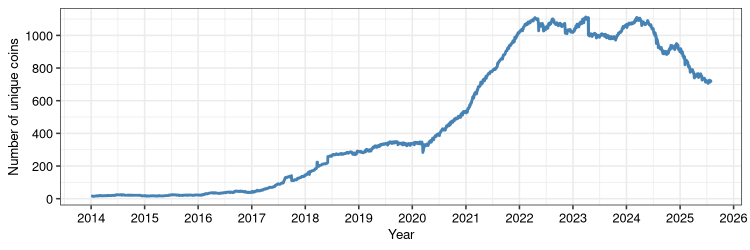
\includegraphics[width=0.8\linewidth,height=\textheight,keepaspectratio]{pictures/timeseries_daily_coins.png}

}

\subcaption{\label{fig-sub1}}

\centering{

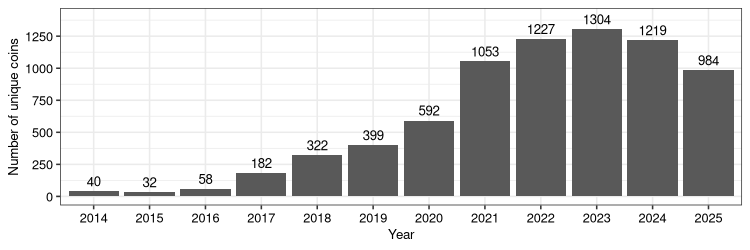
\includegraphics[width=0.8\linewidth,height=\textheight,keepaspectratio]{pictures/coins_per_year.png}

}

\subcaption{\label{fig-sub2}}

}

\caption[Number of cryptocurrencies over
time]{\label{fig-numcoins}\textbf{Number of cryptocurrencies over time.}
Panel A shows the daily time series of the number of unique
cryptocurrencies. Panel B displays the number of unique cryptocurrencies
recorded each year. Both panels correspond to the dataset after applying
the filtering steps (1) to (5), covering the period from January 1,
2014, to July 31, 2025, and including 1,416 unique cryptocurrencies.
Note that coins may enter or exit the market over time.}

\end{figure}%

\section{Sample overview}\label{sample-overview}

After applying all the filters, the resulting sample consists of 973
unique cryptocurrencies and 1,478,936 observations from June 1, 2018, to
July 31, 2025, where a day starts at 00:00:00 UTC. It is important to
mention that the number of cryptocurrencies fluctuates over the entire
period, which results in an unbalanced panel of data. Table
\ref{tbl-cross_section} provides a description of the yearly
cross-sectionional statistics: the sample starts with 254 different
cryptocurrencies in 2018 and peaks in 2023 with 939 unique
cryptocurrencies, before decreasing to 780 in 2025. The minimum daily
cross-section is 121 in 2018, and then increases drastically up to 793
in 2023. For context, at the time of writing, CoinMarketCap tracks
around 19 million cryptocurrencies, and CoinGecko around 19 thousands.
When compared to these numbers, the size of the sample may seem small;
however, it actually covers most of the whole cryptocurrency market
capitalization (see Figure~\ref{fig-samplemarketcap}). The sample period
includes important events in the market, such as

Table \ref{tbl-overview} summarizes the descriptive statistics for the
cryptocurrency daily returns across different subsamples and Bitcoin,
Ethereum, and Ripple, which are the three largest cryptocurrencies in
the sample. Interestingly, the larger samples exhibit a larger
volatility and more pronounced extreme returns, both positive and
negative. Bitcoin shows the lowest mean return during the sample period
(0.16\% per day), though this value very close to that of Ethereum
(0.17\%) and Ripple (0.20\%), and only slightly below other
cryptocurrency subsamples.

\begin{figure}[h]

\centering{

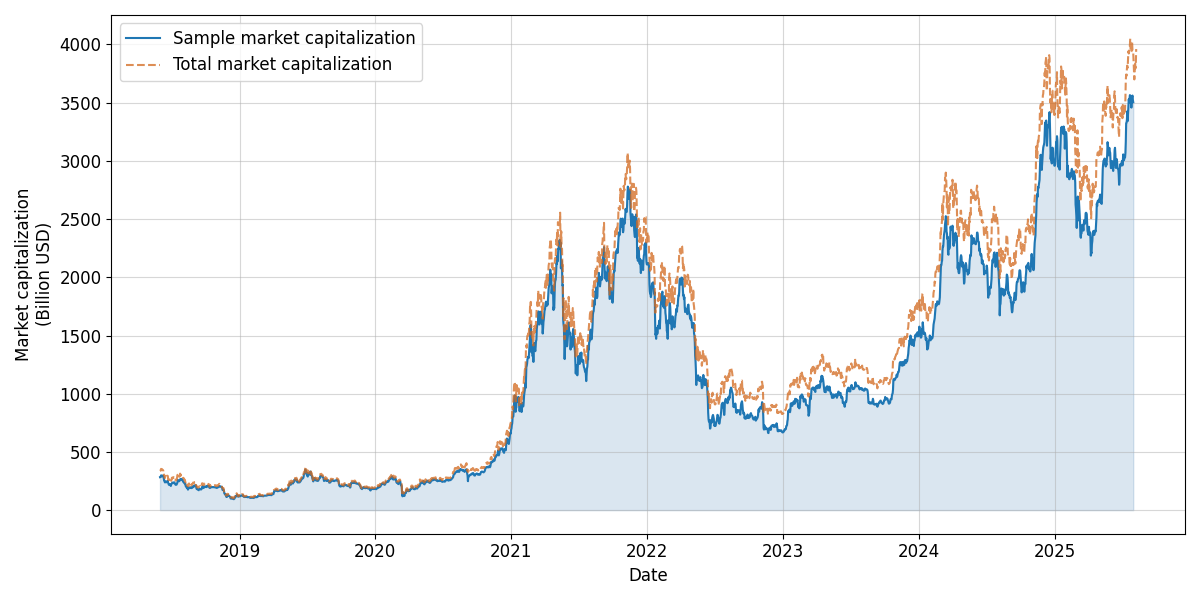
\includegraphics[width=0.8\linewidth,height=\textheight,keepaspectratio]{pictures/sample_marketcap.png}

}

\caption[Cryptocurrency market
capitalization]{\label{fig-samplemarketcap}\textbf{Cryptocurrency market
capitalization}. The figure compares the cryptocurrency market
capitalization in the filtered sample (blue line) with the total market
capitalization (yellow line) from June 1, 2018 to July 31, 2025. Source:
total market capitalization from
\href{https://www.coingecko.com/}{CoinGecko}.}

\end{figure}%

\begin{table}[t]
\footnotesize
\centering
\caption[Cross-section size of the sample]{\textbf{Cross-section size of the sample.} The table repots the number of unique coins per year, as well as the minimum daily cross-section size in the filtered sample.}
\label{tbl-cross_section}
\begin{tabular}{ccccccccc}
\toprule
Year & 2018 & 2019 & 2020 & 2021 & 2022 & 2023 & 2024 & 2025 \\
\midrule
Unique coins & 254 & 337 & 420 & 714 & 938 & 939 & 906 & 780 \\
Min. daily cross-section & 121 & 239 & 207 & 381 & 699 & 793 & 710 & 578 \\
\bottomrule
\end{tabular}
\end{table}

\begin{table}[t]
\centering
\caption[Summary statistics of daily returns]{\textbf{Summary statistics of daily returns.} The table reports summary statistics of daily returns for the filtered sample, the top 100 and top 10 cryptocurrencies ranked by market capitalization, and for Bitcoin, Ethereum, and Ripple individually. Reported statistics include the number of daily observations, the number of unique coins over the sample period, the mean and standard deviation of returns, and the 10th percentile, lower quartile, median, upper quartile, and 90th percentile of the distribution of the returns. The sample period is from June 1, 2018, to July 31, 2025.}
\label{tbl-overview}
\begin{adjustbox}{max width=\textwidth}
\begin{threeparttable}
\begin{tabular}{lccccccccc}
\toprule
 & No. Obs & Unique coins & Mean & Std & P10 & P25 & P50 & P75 & P90 \\
\midrule
Sample & 1,478,936 & 973 & 0.36\% & 12.25\% & -6.83\% & -3.00\% & -0.16\% & 2.57\% & 6.85\% \\
Top 100 & 176,400 & 100 & 0.21\% & 6.93\% & -5.64\% & -2.52\% & -0.03\% & 2.44\% & 5.86\% \\
Top 10 & 24,747 & 10 & 0.25\% & 5.74\% & -4.71\% & -2.00\% & 0.07\% & 2.14\% & 5.07\% \\
Bitcoin & 2,618 & 1 & 0.16\% & 3.33\% & -3.24\% & -1.27\% & 0.09\% & 1.52\% & 3.67\% \\
Ethereum & 2,611 & 1 & 0.17\% & 4.35\% & -4.33\% & -1.77\% & 0.10\% & 2.14\% & 4.88\% \\
Ripple & 2,540 & 1 & 0.20\% & 5.31\% & -4.48\% & -1.87\% & 0.08\% & 1.89\% & 4.70\% \\
\bottomrule
\end{tabular}
\begin{tablenotes}\footnotesize
\item[1] As of July 31, 2025, the top 10 cryptocurrencies are Bitcoin, Ethereum, Ripple, Binance Coin, Solana, Dogecoin, Tron, Cardano, Stellar, and Chainlink.
\end{tablenotes}
\end{threeparttable}
\end{adjustbox}
\end{table}

The sample period spans several major market, economic, and political
events, these include: the start of the COVID-19 pandemic and the
subsequent crypto bubble in 2020-2021, El Salvador adoption of Bitcoin
as legal tender in September 2021, and China's ban on cryptocurrency
exchanges and mining in October 2021. The period also experienced
multiple cryptocurrency exchange hacks\footnote{For example, Binance,
  largest crypto exchange in the world, was hacked in 2019, and KuCoin
  and Crypto.com were hacked in 2020 and 2022, respectively.
  (\citeproc{ref-zhouApplicationEvent2025}{Zhou, 2025})}, and
geopolitical shocks such as the Russia-Ukraine war in February 2022, and
the Palestine-Israel war in October 2023. More recently, in 2024, the
U.S. Secutities and Exchange Commission (SEC) approved the listing and
trading of several crypto spot ETFs in January, and Donald Trump's
election as U.S. president, with Elon Musk playing and important role in
his campaign
(\citeproc{ref-bianchiMispricingRiskCompensation2021}{Bianchi \& Babiak,
2021b}; \citeproc{ref-chenHowEffective2022}{C. Chen \& Liu, 2022};
\citeproc{ref-liuSpotCryptocurrency2024}{S. Liu \& Yang, 2024};
\citeproc{ref-mercikCrosssectionalInteractionsCryptocurrency2025}{Mercik
et al., 2025}; \citeproc{ref-zhouApplicationEvent2025}{Zhou, 2025}).

\section{Characteristic construction and
description}\label{sec-characteristics}

For the analysis, I construct 41 asset-specific characteristics from the
cross-section of 973 cryptocurrencies using data on prices, volume, and
market capitalization. Specifically, I follow the methodology of Bianchi
\& Babiak (\citeproc{ref-bianchiMispricingRiskCompensation2021}{2021b}),
Y. Liu et al. (\citeproc{ref-liuCommonRisk2022}{2022}), and Mercik et
al.
(\citeproc{ref-mercikCrosssectionalInteractionsCryptocurrency2025}{2025})
to construct the set of characteristics widely used in the
cryptocurrency and financial literature, which serve as return
predictors in the empirical analysis. These characteristics are grouped
into six categories: market and size, volatility and risk, trading
activity, liquidity, past returns, and distribution. Table
\ref{tbl-characteristics} summarizes the set of characteristics, while
Appendix \ref{sec-app_characteristics} provides detailed definitions and
construction procedures.

\begin{table}
\centering
\caption[Cryptocurrency characteristics.]{\label{tab:unnamed-chunk-1}\textbf{Cryptocurrency characteristics.} The table presents the 41 cryptocurrency characteristics used as return predictors in the empirical analysis. The characteristics are grouped in six categories: price and size, volatility and risk, trading activity, liquidity, past returns, and distribution. \label{tbl-characteristics}}
\centering
\fontsize{8}{10}\selectfont
\begin{tabular}[t]{l>{\raggedright\arraybackslash}p{10em}l>{\raggedright\arraybackslash}p{27em}}
\toprule
No. & Characteristic & Symbol & Definition\\
\midrule
\addlinespace[0.3em]
\multicolumn{4}{l}{\textbf{Panel A: Price \& size}}\\
\hspace{1em}(1) & Market capitalization & mcap & Last day's market capitalization.\\
\hspace{1em}(2) & Price & prc & Last day's logged closing price.\\
\hspace{1em}(3) & Closeness to the 90-day high & dh90 & Last day's price over the maximum price in the previous 90 days.\\
\addlinespace[0.3em]
\multicolumn{4}{l}{\textbf{Panel B: Volatility \& risk}}\\
\hspace{1em}(4) & Market beta & beta & CAPM market beta, estimated from 30 days of daily returns.\\
\hspace{1em}(5) & Idiosyncratic volatility & ivol & Volatility of CAPM residuals over 30 days of daily returns.\\
\hspace{1em}(6-7) & Realized volatility & rvol\_*d & Realized volatility, calculated from 7 and 30 days of OHCL prices.\\
\hspace{1em}(8) & Return volatility & retvol & Standard deviation of daily returns over 7 days.\\
\hspace{1em}(9) & Value-at-Risk & var & The historical Value-at-Risk at 5\% level over 90 days.\\
\hspace{1em}(10) & Expected Shortfall & es\_5 & The expected shortfall at the 5\% level over 90 days.\\
\hspace{1em}(11) & Price delay & delay & Improvement in \(R^2\) after adding lagged one-and two-day market excecss return to the CAPM.\\
\addlinespace[0.3em]
\multicolumn{4}{l}{\textbf{Panel C: Trading activity}}\\
\hspace{1em}(12) & Trading volume & volume & Last day's daily trading volume in US dollars.\\
\hspace{1em}(13) & Average volume & volume\_*d & Mean volume over the past 7 and 30 days.\\
\hspace{1em}(15) & Turnover & turn & The last day's trading volume over current market capitalization.\\
\hspace{1em}(16) & Average 7-day turnover & turn\_7d & Mean turnover over the past 7 days.\\
\hspace{1em}(17) & Turnover volatility & std\_turn & Turnover volatility over the past 30 days.\\
\hspace{1em}(18) & Trading volume volatility & std\_vol & Volume's logged volatility over the past 30 days.\\
\hspace{1em}(19) & Volume's coefficient of variation & cv\_vol & Volume's volatility over its mean in the previous 30 days.\\
\addlinespace[0.3em]
\multicolumn{4}{l}{\textbf{Panel D: Liquidity}}\\
\hspace{1em}(20) & Bid-ask spread & bidask & Mean estimated bid-ask spread calculated over the past 30 days.\\
\hspace{1em}(21) & Illiquidity & illiq & Mean absolute daily return over trading volume over the past 30 days.\\
\hspace{1em}(22) & Standardized abnormal turnover & sat & Last day's turnover minus its 30-day average, divided its volatility over 30 days.\\
\hspace{1em}(23) & De-trended turnover & dto & De-trended turnover minus the value-weighted daily market turnover.\\
\hspace{1em}(24) & Volume Shock 15-day & volsh\_15d & Log deviation of trading volume from its rolling 15-day average.\\
\hspace{1em}(25) & Voume Shock 30-day & volsh\_30d & Log deviation of trading volume from its rolling 30-day average.\\
\addlinespace[0.3em]
\multicolumn{4}{l}{\textbf{Panel E: Past returns}}\\
\hspace{1em}(26) & Daily reversal & r2\_1 & Return on the previous trading day.\\
\hspace{1em}(27-30) & Momentum & r*\_1 & 7, 14, 21, and 30-day cumulative return ending 1 day before the prediction date.\\
\hspace{1em}(31) & Intermediate momentum & r30\_14 & Cumulative return from 30 to 14 days before the prediction date.\\
\hspace{1em}(32) & Long-term reversal & r180\_60 & Cumulative return from 180 to 60 days before the prediction date.\\
\hspace{1em}(33) & CAPM alpha & alpha & CAPM intercept, estimated from 30 days of daily returns.\\
\addlinespace[0.3em]
\multicolumn{4}{l}{\textbf{Panel F: Distribution}}\\
\hspace{1em}(34-35) & Skewness & skew\_*d & Skewness of the daily return distribution over a 7-and 30-day period.\\
\hspace{1em}(36-37) & Kurtosis & kurt\_*d & Kurtosis of the daily return distribution over a 7-and 30-day period.\\
\hspace{1em}(38-39) & Maximum daily return & maxret\_*d & The maximum daily return in the past 7-and 30 days.\\
\hspace{1em}(40-41) & Minimum daily return & minret\_*d & The minimum daily return in the past 7-and 30 days.\\
\bottomrule
\end{tabular}
\end{table}

\section{Observable risk factors}\label{observable-risk-factors}

In addition to the set of characteristics described above, I construct a
set of observable risk factors. In the asset pricing literature, the
convention is to analyze the risk compensation of asset returns using
factor-mimicking portfolio (e.g.
\citeproc{ref-carhartPersistenceMutual1997}{Carhart, 1997};
\citeproc{ref-famaCommonRisk1993}{Fama \& French, 1993},
\citeproc{ref-famaFivefactorAsset2015}{2015}). This typically involves
sorting assets cross-sectionally into quintiles based on a specific
characteristic and forming a factor return, calculated as the difference
in returns between the top and the bottom quintiles. This approach
replicates a strategy that buys the portfolio of assets with high values
of a particular characteristic (long), and sells the portfolio with the
lowest values (short).

Building on this methodology, I construct a series of observable risk
factors that prior literature have shown to explain the cross-section of
cryptocurrency returns. Specifically, I include the market, size,
momentum, liquidity, and volatility factors, following Y. Liu et al.
(\citeproc{ref-liuCommonRisk2022}{2022}), Bianchi \& Babiak
(\citeproc{ref-bianchi2021factor}{2021a}), and Lan \& Frömmel
(\citeproc{ref-lanRiskFactors2025}{2025}). Details on their construction
are provided in Appendix~\ref{sec-obs_factors}. As described in
Section~\ref{sec-methodology}, the IPCA allows for the inclusion of
pre-specified factors within the more general model specification. I
make use of this feature and pre-specify the observable factors in the
IPCA model, with and without using asset-characteristics to instrument
for dynamic loadings.

\bookmarksetup{startatroot}

\chapter{Results}\label{results}

Write this in the following section of ``Empirical application'' or This
is for the model: 7. (Still undecisive) Minimum cross-section. Following
the criterion by Kelly, I Convert variables in the -0.5 - 0.5 range

The sample period ranges from January 1st, 2014, to May 31st, 2025.

Implemented in python, based on the IPCA python code of Seth Pruitt
\footnote{See https://sethpruitt.net/research/.} and the \texttt{ipca}
python package of Buechner \& Bybee (\citeproc{ref-ipca}{2019})
\footnote{See https://bkelly-lab.github.io/ipca/.}.

Following Kelly et al.
(\citeproc{ref-kellyCharacteristicsAre2019}{2019}), I cross-sectionally
transform the instrument variables period-by-period in the following
manner: first,

\textbf{Important}: mention the shift of characteristics: the
conditional APT of Kelly, Pruitt, Su (JFE 2019) says that the
characteristics known at Date=d-1 determine the exposures associated
with the returns realized at Date=d; hence, here we should have shifted
the characteristics in Z relative to the returns in R

This is a template of the table of the results of the IPCA model. I need
to add a caption to the table. Here I reference Table
\ref{tbl-ipca_results}.

\begin{table}
\centering
\small
%\fontsize{9.0pt}{10.8pt}\selectfont
\caption[Results of IPCA regression]%
{%
\textbf{Results of IPCA regression.}
Model Performance. Panel A and B report total and predictive $R^2$ in percent for the restricted ($\Gamma_\alpha = 0$) and unrestricted ($\Gamma_\alpha \neq 0$) IPCA model for $K$ number of factors on daily and weekly data, respectively. Panel C reports the corresponding total and predictive $R^2$ for a simple PCA model on weekly data.
}
\label{tbl-ipca_results}
\begin{tabular}{lcccc}
\toprule
 &  & \multicolumn{3}{c}{K } \\
\cmidrule(lr){3-5}
 &  & \(K = 3\) & \(K = 5\) & \(K = 8\) \\
\midrule\addlinespace[2.5pt]
\multicolumn{5}{l}{Panel C: PCA on weekly data} \\[2.5pt]
\midrule\addlinespace[2.5pt]
\(R^{2}_{\text{Total}}\) &  & 0.0000 & 0.0000 & 0.0000 \\
\(R^{2}_{\text{Predictive}}\) &  & 0.0000 & 0.0000 & 0.0000 \\
\midrule\addlinespace[2.5pt]
\multicolumn{5}{l}{Panel B: IPCA on weekly data} \\[2.5pt]
\midrule\addlinespace[2.5pt]
\(R^{2}_{\text{Total}}\) & \(\Gamma_{\alpha} = 0\) & 0.2625 & 0.2817 & 0.2934 \\
 & \(\Gamma_{\alpha} \neq 0\) & 0.2661 & 0.2826 & 0.2937 \\
\(R^{2}_{\text{Predictive}}\) & \(\Gamma_{\alpha} = 0\) & 0.1725 & 0.1551 & 0.1511 \\
 & \(\Gamma_{\alpha} \neq 0\) & 0.1719 & 0.1584 & 0.1554 \\
\midrule\addlinespace[2.5pt]
\multicolumn{5}{l}{Panel A: IPCA on daily data} \\[2.5pt]
\midrule\addlinespace[2.5pt]
\(R^{2}_{\text{Total}}\) & \(\Gamma_{\alpha} = 0\) & 0.2301 & 0.2509 & 0.2681 \\
 & \(\Gamma_{\alpha} \neq 0\) & 0.2322 & 0.2524 & 0.2690 \\
\(R^{2}_{\text{Predictive}}\) & \(\Gamma_{\alpha} = 0\) & -0.3904 & -0.4082 & -0.4169 \\
 & \(\Gamma_{\alpha} \neq 0\) & -0.3857 & -0.4055 & -0.4156 \\
\bottomrule
\end{tabular}
\end{table}

Some test for quarto and latex

Quarto: 1. Sees the caption line after the table. 2. Wraps the
\texttt{tabular} inside a LaTeX \texttt{table} environment. 3. Adds
\texttt{\textbackslash{}caption\{Some\ letters\ with\ LaTeX\}} and
\texttt{\textbackslash{}label\{tbl-letters\}} automatically. 4. Gives it
a table number and puts it in the List of Tables.

\begin{center}\rule{0.5\linewidth}{0.5pt}\end{center}

\textbf{Inline LaTeX way inside Quarto}\\
Here we see the summary statistics in Table \ref{tbl-letters}.

\begin{table}

\caption{\label{tbl-letters}Some letters with LaTeX}

\centering{

\centering

\begin{tabular}{lll}
A & B & C \\
D & E & F \\
\end{tabular}

}

\end{table}%

\bookmarksetup{startatroot}

\chapter{Conclusion}\label{conclusion}

\bookmarksetup{startatroot}

\chapter*{References}\label{references}
\addcontentsline{toc}{chapter}{References}

\markboth{References}{References}

\phantomsection\label{refs}
\begin{CSLReferences}{1}{0}
\bibitem[\citeproctext]{ref-alexanderCriticalInvestigation2020}
Alexander, C., \& Dakos, M. (2020). A critical investigation of
cryptocurrency data and analysis. \emph{Quantitative Finance},
\emph{20}(2), 173--188.
\url{https://doi.org/10.1080/14697688.2019.1641347}

\bibitem[\citeproctext]{ref-Quarto_2025}
Allaire, J. J., Teague, C., Scheidegger, C., Xie, Y., Dervieux, C., \&
Woodhull, G. (2025). \emph{{Quarto}} (Version 1.7) {[}Computer
software{]}. \url{https://doi.org/10.5281/zenodo.5960048}

\bibitem[\citeproctext]{ref-amihudIlliquidityStock2002}
Amihud, Y. (2002). Illiquidity and stock returns: cross-section and
time-series effects. \emph{Journal of Financial Markets}, \emph{5}(1),
31--56. \url{https://doi.org/10.1016/S1386-4181(01)00024-6}

\bibitem[\citeproctext]{ref-angCrossSectionVolatility2006}
Ang, A., Hodrick, R. J., Xing, Y., \& Zhang, X. (2006). The
Cross-Section of Volatility and Expected Returns. \emph{The Journal of
Finance}, \emph{61}(1), 259--299.
\url{https://doi.org/10.1111/j.1540-6261.2006.00836.x}

\bibitem[\citeproctext]{ref-bidask}
Ardia, D., Guidotti, E., \& Kroencke, T. A. (2024). Efficient estimation
of bid--ask spreads from open, high, low, and close prices.
\emph{Journal of Financial Economics}, \emph{161}, 103916.
\url{https://doi.org/10.1016/j.jfineco.2024.103916}

\bibitem[\citeproctext]{ref-asadovGreaterStability2023}
Asadov, A., Yildirim, R., \& Masih, M. (2023). Toward greater stability
in stablecoins: Empirical evidence from an analysis of precious metals.
\emph{Borsa Istanbul Review}, \emph{23}(5), 1152--1172.
\url{https://doi.org/10.1016/j.bir.2023.07.004}

\bibitem[\citeproctext]{ref-babiakVariationsTrading2022}
Babiak, M., \& Erdis, M. B. (2022). \emph{Variations in Trading
Activity, Costly Arbitrage, and Cryptocurrency Returns} (SSRN Scholarly
Paper 4291073). Social Science Research Network.
\url{https://doi.org/10.2139/ssrn.4291073}

\bibitem[\citeproctext]{ref-baekBitcoinsInvestment2015}
Baek, C., \& Elbeck, M. (2015). Bitcoins as an investment or speculative
vehicle? A first look. \emph{Applied Economics Letters}, \emph{22}(1),
30--34. \url{https://doi.org/10.1080/13504851.2014.916379}

\bibitem[\citeproctext]{ref-baurVolatilityBitcoin2021}
Baur, D. G., \& Dimpfl, T. (2021). The volatility of Bitcoin and its
role as a medium of exchange and a store of value. \emph{Empirical
Economics}, \emph{61}(5), 2663--2683.
\url{https://doi.org/10.1007/s00181-020-01990-5}

\bibitem[\citeproctext]{ref-baurCryptoSafe2021}
Baur, D. G., \& Hoang, L. T. (2021). A crypto safe haven against
Bitcoin. \emph{Finance Research Letters}, \emph{38}, 101431.
\url{https://doi.org/10.1016/j.frl.2020.101431}

\bibitem[\citeproctext]{ref-baurBitcoinMedium2018}
Baur, D. G., Hong, K., \& Lee, A. D. (2018). Bitcoin: Medium of exchange
or speculative assets? \emph{Journal of International Financial Markets,
Institutions and Money}, \emph{54}, 177--189.
\url{https://doi.org/10.1016/j.intfin.2017.12.004}

\bibitem[\citeproctext]{ref-bianchi2021factor}
Bianchi, D., \& Babiak, M. (2021a). A factor model for cryptocurrency
returns. \emph{CERGE-EI Working Paper Series}, \emph{710}.

\bibitem[\citeproctext]{ref-bianchiMispricingRiskCompensation2021}
Bianchi, D., \& Babiak, M. (2021b). \emph{Mispricing and Risk
Compensation in Cryptocurrency Returns} (SSRN Scholarly Paper 3935934).
Social Science Research Network.
\url{https://doi.org/10.2139/ssrn.3935934}

\bibitem[\citeproctext]{ref-bouriForecastingReturns2022}
Bouri, E., Christou, C., \& Gupta, R. (2022). Forecasting returns of
major cryptocurrencies: Evidence from regime-switching factor models.
\emph{Finance Research Letters}, \emph{49}, 103193.
\url{https://doi.org/10.1016/j.frl.2022.103193}

\bibitem[\citeproctext]{ref-ipca}
Buechner, M., \& Bybee, L. (2019). \emph{{ipca}: Instrumented principal
components analysis} {[}Computer software{]}.
\url{https://github.com/bkelly-lab/ipca}

\bibitem[\citeproctext]{ref-carhartPersistenceMutual1997}
Carhart, M. M. (1997). On Persistence in Mutual Fund Performance.
\emph{The Journal of Finance}, \emph{52}(1), 57--82.
\url{https://doi.org/10.1111/j.1540-6261.1997.tb03808.x}

\bibitem[\citeproctext]{ref-chamberlainArbitrageFactor1983}
Chamberlain, G., \& Rothschild, M. (1983). Arbitrage, Factor Structure,
and Mean-Variance Analysis on Large Asset Markets. \emph{Econometrica},
\emph{51}(5), 1281--1304. \url{https://doi.org/10.2307/1912275}

\bibitem[\citeproctext]{ref-chenOpenSource2021}
Chen, A. Y., \& Zimmermann, T. (2021). \emph{Open Source Cross-Sectional
Asset Pricing} (SSRN Scholarly Paper 3604626). Social Science Research
Network. \url{https://doi.org/10.2139/ssrn.3604626}

\bibitem[\citeproctext]{ref-chenHowEffective2022}
Chen, C., \& Liu, L. (2022). How effective is China's cryptocurrency
trading ban? \emph{Finance Research Letters}, \emph{46}, 102429.
\url{https://doi.org/10.1016/j.frl.2021.102429}

\bibitem[\citeproctext]{ref-chenSemiparametricConditional2022}
Chen, Q., Roussanov, N. L., \& Wang, X. (2022). \emph{Semiparametric
Conditional Factor Models in Asset Pricing} (SSRN Scholarly Paper
3984633). Social Science Research Network.
\url{https://doi.org/10.2139/ssrn.3984633}

\bibitem[\citeproctext]{ref-chenCommonRisk2024}
Chen, Z., Roussanov, N. L., Wang, X., \& Zou, D. (2024). \emph{Common
Risk Factors in the Returns on Stocks, Bonds (and Options), Redux} (SSRN
Scholarly Paper 4703281). Social Science Research Network.
\url{https://doi.org/10.2139/ssrn.4703281}

\bibitem[\citeproctext]{ref-cochrane2009asset}
Cochrane, J. H. (2005). \emph{Asset pricing: Revised edition}. Princeton
University Press.

\bibitem[\citeproctext]{ref-cochranePresidentialAddress2011}
Cochrane, J. H. (2011). Presidential Address: Discount Rates. \emph{The
Journal of Finance}, \emph{66}(4), 1047--1108.
\url{https://doi.org/10.1111/j.1540-6261.2011.01671.x}

\bibitem[\citeproctext]{ref-coinbaseWhatWrapped}
Coinbase. (n.d.). \emph{What is wrapped crypto?} Retrieved August 6,
2025, from
\url{https://www.coinbase.com/learn/your-crypto/what-is-wrapped-crypto}

\bibitem[\citeproctext]{ref-coingecko2025Q2}
CoinGecko. (n.d.). \emph{2025 Q2 Crypto Industry Report}. CoinGecko
Cryptocurrency Reports. Retrieved July 25, 2025, from
\url{https://www.coingecko.com/en/publications/reports}

\bibitem[\citeproctext]{ref-congValuePremium2022}
Cong, L. W., Karolyi, G. A., Tang, K., \& Zhao, W. (2022). \emph{Value
Premium, Network Adoption, and Factor Pricing of Crypto Assets} (SSRN
Scholarly Paper 3985631). Social Science Research Network.
\url{https://doi.org/10.2139/ssrn.3985631}

\bibitem[\citeproctext]{ref-conlonAreCryptocurrencies2020}
Conlon, T., Corbet, S., \& McGee, R. J. (2020). Are cryptocurrencies a
safe haven for equity markets? An international perspective from the
COVID-19 pandemic. \emph{Research in International Business and
Finance}, \emph{54}, 101248.
\url{https://doi.org/10.1016/j.ribaf.2020.101248}

\bibitem[\citeproctext]{ref-connorPerformanceMeasurement1986}
Connor, G., \& Korajczyk, R. A. (1986). Performance measurement with the
arbitrage pricing theory: A new framework for analysis. \emph{Journal of
Financial Economics}, \emph{15}(3), 373--394.
\url{https://doi.org/10.1016/0304-405X(86)90027-9}

\bibitem[\citeproctext]{ref-datarLiquidityStock1998}
Datar, V. T., Y. Naik, N., \& Radcliffe, R. (1998). Liquidity and stock
returns: An alternative test. \emph{Journal of Financial Markets},
\emph{1}(2), 203--219.
\url{https://doi.org/10.1016/S1386-4181(97)00004-9}

\bibitem[\citeproctext]{ref-dwyerEconomicsBitcoin2015}
Dwyer, G. P. (2015). The economics of Bitcoin and similar private
digital currencies. \emph{Journal of Financial Stability}, \emph{17},
81--91. \url{https://doi.org/10.1016/j.jfs.2014.11.006}

\bibitem[\citeproctext]{ref-famaCommonRisk1993}
Fama, E. F., \& French, K. R. (1993). Common risk factors in the returns
on stocks and bonds. \emph{Journal of Financial Economics},
\emph{33}(1), 3--56. \url{https://doi.org/10.1016/0304-405X(93)90023-5}

\bibitem[\citeproctext]{ref-famaFivefactorAsset2015}
Fama, E. F., \& French, K. R. (2015). A five-factor asset pricing model.
\emph{Journal of Financial Economics}, \emph{116}(1), 1--22.
\url{https://doi.org/10.1016/j.jfineco.2014.10.010}

\bibitem[\citeproctext]{ref-fengTamingFactor2020}
Feng, G., Giglio, S., \& Xiu, D. (2020). Taming the Factor Zoo: A Test
of New Factors. \emph{The Journal of Finance}, \emph{75}(3), 1327--1370.
\url{https://doi.org/10.1111/jofi.12883}

\bibitem[\citeproctext]{ref-financialstabilityboardAddressingRegulatory2020}
Financial Stability Board. (2020). \emph{Addressing the regulatory,
supervisory and oversight challenges raised by {``global stablecoin''}
arrangements: Consultative document}.
\url{https://www.fsb.org/2020/04/addressing-the-regulatory-supervisory-and-oversight-challenges-raised-by-global-stablecoin-arrangements-consultative-document/}

\bibitem[\citeproctext]{ref-garfinkelMeasuringInvestors2009}
Garfinkel, J. A. (2009). Measuring Investors' Opinion Divergence.
\emph{Journal of Accounting Research}, \emph{47}(5), 1317--1348.
\url{https://doi.org/10.1111/j.1475-679X.2009.00344.x}

\bibitem[\citeproctext]{ref-garfinkelDisagreementReturns}
Garfinkel, J. A., Hsiao, L., \& Hu, D. (n.d.). Disagreement and returns:
The case of cryptocurrencies. \emph{Financial Management},
\emph{n/a}(n/a). \url{https://doi.org/10.1111/fima.12491}

\bibitem[\citeproctext]{ref-george52WeekHigh2004}
George, T. J., \& Hwang, C.-Y. (2004). The 52-Week High and Momentum
Investing. \emph{The Journal of Finance}, \emph{59}(5), 2145--2176.
\url{https://doi.org/10.1111/j.1540-6261.2004.00695.x}

\bibitem[\citeproctext]{ref-glaserBitcoinAsset2014}
Glaser, F., Zimmermann, K., Haferkorn, M., Weber, M. C., \& Siering, M.
(2014). \emph{Bitcoin - Asset or Currency? Revealing Users' Hidden
Intentions} (SSRN Scholarly Paper 2425247). Social Science Research
Network. \url{https://papers.ssrn.com/abstract=2425247}

\bibitem[\citeproctext]{ref-harris2020array}
Harris, C. R., Millman, K. J., Walt, S. J. van der, Gommers, R.,
Virtanen, P., Cournapeau, D., Wieser, E., Taylor, J., Berg, S., Smith,
N. J., Kern, R., Picus, M., Hoyer, S., Kerkwijk, M. H. van, Brett, M.,
Haldane, A., Río, J. F. del, Wiebe, M., Peterson, P., \ldots{} Oliphant,
T. E. (2020). Array programming with {NumPy}. \emph{Nature},
\emph{585}(7825), 357--362.
\url{https://doi.org/10.1038/s41586-020-2649-2}

\bibitem[\citeproctext]{ref-harveyLuckyFactors2021}
Harvey, C. R., \& Liu, Y. (2021). Lucky factors. \emph{Journal of
Financial Economics}, \emph{141}(2), 413--435.
\url{https://doi.org/10.1016/j.jfineco.2021.04.014}

\bibitem[\citeproctext]{ref-hoangHowStable2024}
Hoang, L. T., \& Baur, D. G. (2024). How stable are stablecoins?
\emph{The European Journal of Finance}, \emph{30}(16), 1984--2000.
\url{https://doi.org/10.1080/1351847X.2021.1949369}

\bibitem[\citeproctext]{ref-houMarketFrictions2005}
Hou, K., \& Moskowitz, T. J. (2005). Market Frictions, Price Delay, and
the Cross-Section of Expected Returns. \emph{The Review of Financial
Studies}, \emph{18}(3), 981--1020.
\url{https://doi.org/10.1093/rfs/hhi023}

\bibitem[\citeproctext]{ref-houReplicatingAnomalies2020}
Hou, K., Xue, C., \& Zhang, L. (2020). Replicating Anomalies. \emph{The
Review of Financial Studies}, \emph{33}(5), 2019--2133.
\url{https://doi.org/10.1093/rfs/hhy131}

\bibitem[\citeproctext]{ref-Hunter:2007}
Hunter, J. D. (2007). Matplotlib: A 2D graphics environment.
\emph{Computing in Science \& Engineering}, \emph{9}(3), 90--95.
\url{https://doi.org/10.1109/MCSE.2007.55}

\bibitem[\citeproctext]{ref-huynhWhenElon2023}
Huynh, T. L. D. (2023). When Elon Musk Changes his Tone, Does Bitcoin
Adjust Its Tune? \emph{Computational Economics}, \emph{62}(2), 639--661.
\url{https://doi.org/10.1007/s10614-021-10230-6}

\bibitem[\citeproctext]{ref-jungCommonFactors2024}
Jung, W., \& Park, H. (2024). Common factors in the returns on
cryptocurrencies. \emph{Finance Research Letters}, \emph{65}, 105485.
\url{https://doi.org/10.1016/j.frl.2024.105485}

\bibitem[\citeproctext]{ref-kalachevaDetectingRug2025}
Kalacheva, A., Kuznetsov, P., Vodolazov, I., \& Yanovich, Y. (2025).
Detecting Rug Pulls in Decentralized Exchanges: The Rise of Meme Coins.
\emph{Blockchain: Research and Applications}, 100336.
\url{https://doi.org/10.1016/j.bcra.2025.100336}

\bibitem[\citeproctext]{ref-kellyCharacteristicsAre2019}
Kelly, B. T., Pruitt, S., \& Su, Y. (2019). Characteristics are
covariances: A unified model of risk and return. \emph{Journal of
Financial Economics}, \emph{134}(3), 501--524.
\url{https://doi.org/10.1016/j.jfineco.2019.05.001}

\bibitem[\citeproctext]{ref-kellyInstrumentedPrincipal2020}
Kelly, B. T., Pruitt, S., \& Su, Y. (2020). \emph{Instrumented Principal
Component Analysis} (SSRN Scholarly Paper 2983919). Social Science
Research Network. \url{https://doi.org/10.2139/ssrn.2983919}

\bibitem[\citeproctext]{ref-kleinBitcoinNot2018}
Klein, T., Pham Thu, H., \& Walther, T. (2018). Bitcoin is not the New
Gold -- A comparison of volatility, correlation, and portfolio
performance. \emph{International Review of Financial Analysis},
\emph{59}, 105--116. \url{https://doi.org/10.1016/j.irfa.2018.07.010}

\bibitem[\citeproctext]{ref-moments}
Komsta, L., \& Novomestky, F. (2022). \emph{{moments}: Moments,
cumulants, skewness, kurtosis and related tests}.
\url{https://doi.org/10.32614/CRAN.package.moments}

\bibitem[\citeproctext]{ref-lanRiskFactors2025}
Lan, T., \& Frömmel, M. (2025). Risk factors in cryptocurrency pricing.
\emph{International Review of Financial Analysis}, \emph{105}, 104389.
\url{https://doi.org/10.1016/j.irfa.2025.104389}

\bibitem[\citeproctext]{ref-lewellenConditionalCAPM2006}
Lewellen, J., \& Nagel, S. (2006). The conditional CAPM does not explain
asset-pricing anomalies. \emph{Journal of Financial Economics},
\emph{82}(2), 289--314.
\url{https://doi.org/10.1016/j.jfineco.2005.05.012}

\bibitem[\citeproctext]{ref-liebiThereValue2020}
Liebi, L. (2020). \emph{Is There a Value Premium in Cryptoasset
Markets?} (SSRN Scholarly Paper 3718684). Social Science Research
Network. \url{https://doi.org/10.2139/ssrn.3718684}

\bibitem[\citeproctext]{ref-lintnerValuationRisk1965}
Lintner, J. (1965). The Valuation of Risk Assets and the Selection of
Risky Investments in Stock Portfolios and Capital Budgets. \emph{The
Review of Economics and Statistics}, \emph{47}(1), 13--37.
\url{https://doi.org/10.2307/1924119}

\bibitem[\citeproctext]{ref-liuSpotCryptocurrency2024}
Liu, S., \& Yang, C. (2024). Spot cryptocurrency ETFs: Crypto investment
products or stepping stones toward tokenization. \emph{Finance Research
Letters}, \emph{69}, 106150.
\url{https://doi.org/10.1016/j.frl.2024.106150}

\bibitem[\citeproctext]{ref-liuCommonRisk2020}
Liu, W., Liang, X., \& Cui, G. (2020). Common risk factors in the
returns on cryptocurrencies. \emph{Economic Modelling}, \emph{86},
299--305. \url{https://doi.org/10.1016/j.econmod.2019.09.035}

\bibitem[\citeproctext]{ref-liuRisksReturns2021}
Liu, Y., \& Tsyvinski, A. (2021). Risks and Returns of Cryptocurrency.
\emph{The Review of Financial Studies}, \emph{34}(6), 2689--2727.
\url{https://doi.org/10.1093/rfs/hhaa113}

\bibitem[\citeproctext]{ref-liuCommonRisk2022}
Liu, Y., Tsyvinski, A., \& Wu, X. (2022). Common Risk Factors in
Cryptocurrency. \emph{The Journal of Finance}, \emph{77}(2), 1133--1177.
\url{https://doi.org/10.1111/jofi.13119}

\bibitem[\citeproctext]{ref-llorenteDynamicVolumeReturn2002}
Llorente, G., Michaely, R., Saar, G., \& Wang, J. (2002). Dynamic
Volume-Return Relation of Individual Stocks. \emph{The Review of
Financial Studies}, \emph{15}(4), 1005--1047.
\url{https://doi.org/10.1093/rfs/15.4.1005}

\bibitem[\citeproctext]{ref-meiklejohnFistfulBitcoins2013}
Meiklejohn, S., Pomarole, M., Jordan, G., Levchenko, K., McCoy, D.,
Voelker, G. M., \& Savage, S. (2013). A fistful of bitcoins:
characterizing payments among men with no names. \emph{Proceedings of
the 2013 Conference on Internet Measurement Conference}, 127--140.
\url{https://doi.org/10.1145/2504730.2504747}

\bibitem[\citeproctext]{ref-mercikCrosssectionalInteractionsCryptocurrency2025}
Mercik, A., Będowska-Sójka, B., Karim, S., \& Zaremba, A. (2025).
Cross-sectional interactions in cryptocurrency returns.
\emph{International Review of Financial Analysis}, \emph{97}, 103809.
\url{https://doi.org/10.1016/j.irfa.2024.103809}

\bibitem[\citeproctext]{ref-mertonIntertemporalCapital1973}
Merton, R. C. (1973). An Intertemporal Capital Asset Pricing Model.
\emph{Econometrica}, \emph{41}(5), 867--887.
\url{https://doi.org/10.2307/1913811}

\bibitem[\citeproctext]{ref-nakamoto2008bitcoin}
Nakamoto, S. (2008). \emph{Bitcoin: A peer-to-peer electronic cash
system}.

\bibitem[\citeproctext]{ref-nicasMileiux24Melania2025}
Nicas, J., Nicas, D. Y.-B. J., Argentina, who covers, Yaffe-Bellany,
reported from R. de J. D., Industry, W. C. the C., \& Francisco,
reported from S. (2025, February 28). Milei, \$Melania and Memecoins:
Unraveling Argentina's Crypto Fiasco. \emph{The New York Times}.
\url{https://www.nytimes.com/2025/02/28/world/americas/argentina-crypto-scandal-president.html}

\bibitem[\citeproctext]{ref-PerformanceAnalytics}
Peterson, B. G., \& Carl, P. (2024). \emph{{PerformanceAnalytics}:
Econometric tools for performance and risk analysis}.
\url{https://doi.org/10.32614/CRAN.package.PerformanceAnalytics}

\bibitem[\citeproctext]{ref-rstudio}
Posit team. (2025). \emph{{RStudio}: Integrated development environment
for r}. Posit Software, PBC. \url{http://www.posit.co/}

\bibitem[\citeproctext]{ref-python}
Python Software Foundation. (2025). \emph{Python programming language}
(Version 3.13.5) {[}Computer software{]}. \url{https://www.python.org/}

\bibitem[\citeproctext]{ref-base}
R Core Team. (2025). \emph{R: A language and environment for statistical
computing}. R Foundation for Statistical Computing.
\url{https://www.R-project.org/}

\bibitem[\citeproctext]{ref-rossArbitrageTheory1976}
Ross, S. A. (1976). The arbitrage theory of capital asset pricing.
\emph{Journal of Economic Theory}, \emph{13}(3), 341--360.
\url{https://doi.org/10.1016/0022-0531(76)90046-6}

\bibitem[\citeproctext]{ref-quantmod}
Ryan, J. A., \& Ulrich, J. M. (2025). \emph{{quantmod}: Quantitative
financial modelling framework}.
\url{https://doi.org/10.32614/CRAN.package.quantmod}

\bibitem[\citeproctext]{ref-sharpeCapitalAsset1964}
Sharpe, W. F. (1964). Capital Asset Prices: A Theory of Market
Equilibrium under Conditions of Risk. \emph{The Journal of Finance},
\emph{19}(3), 425--442. \url{https://doi.org/10.2307/2977928}

\bibitem[\citeproctext]{ref-pcaMethods}
Stacklies, W., Redestig, H., Scholz, M., Walther, D., \& Selbig, J.
(2007). pcaMethods -- a bioconductor package providing PCA methods for
incomplete data. \emph{Bioinformatics}, \emph{23}, 1164--1167.

\bibitem[\citeproctext]{ref-reback2020pandas}
The pandas development team. (2020). \emph{Pandas-dev/pandas: pandas}
{[}Computer software{]}. Zenodo.
\url{https://doi.org/10.5281/zenodo.3509134}

\bibitem[\citeproctext]{ref-vasudevaCryptocurrencyInvestment2023}
Vasudeva, S. (2023). Cryptocurrency as an investment or speculation: a
bibliometric review study. \emph{Business Analyst Journal},
\emph{44}(1), 34--50. \url{https://doi.org/10.1108/BAJ-07-2022-0008}

\bibitem[\citeproctext]{ref-slider}
Vaughan, D. (2024). \emph{{slider}: Sliding window functions}.
\url{https://doi.org/10.32614/CRAN.package.slider}

\bibitem[\citeproctext]{ref-vidal-tomasWhichCryptocurrency2022}
Vidal-Tomás, D. (2022). Which cryptocurrency data sources should
scholars use? \emph{International Review of Financial Analysis},
\emph{81}, 102061. \url{https://doi.org/10.1016/j.irfa.2022.102061}

\bibitem[\citeproctext]{ref-2020SciPy-NMeth}
Virtanen, P., Gommers, R., Oliphant, T. E., Haberland, M., Reddy, T.,
Cournapeau, D., Burovski, E., Peterson, P., Weckesser, W., Bright, J.,
van der Walt, S. J., Brett, M., Wilson, J., Millman, K. J., Mayorov, N.,
Nelson, A. R. J., Jones, E., Kern, R., Larson, E., \ldots{} SciPy 1.0
Contributors. (2020). {{SciPy} 1.0: Fundamental Algorithms for
Scientific Computing in Python}. \emph{Nature Methods}, \emph{17},
261--272. \url{https://doi.org/10.1038/s41592-019-0686-2}

\bibitem[\citeproctext]{ref-wangAreStablecoins2020}
Wang, G.-J., Ma, X., \& Wu, H. (2020). Are stablecoins truly
diversifiers, hedges, or safe havens against traditional
cryptocurrencies as their name suggests? \emph{Research in International
Business and Finance}, \emph{54}, 101225.
\url{https://doi.org/10.1016/j.ribaf.2020.101225}

\bibitem[\citeproctext]{ref-tidyverse}
Wickham, H., Averick, M., Bryan, J., Chang, W., McGowan, L. D.,
François, R., Grolemund, G., Hayes, A., Henry, L., Hester, J., Kuhn, M.,
Pedersen, T. L., Miller, E., Bache, S. M., Müller, K., Ooms, J.,
Robinson, D., Seidel, D. P., Spinu, V., \ldots{} Yutani, H. (2019).
Welcome to the {tidyverse}. \emph{Journal of Open Source Software},
\emph{4}(43), 1686. \url{https://doi.org/10.21105/joss.01686}

\bibitem[\citeproctext]{ref-yaffe-bellanyDigitalCoin2024}
Yaffe-Bellany, D. (2024, July 27). A Digital Coin Based on Baby Trump?
Yup. \emph{The New York Times}.
\url{https://www.nytimes.com/2024/07/27/technology/memecoins-crypto-surge.html}

\bibitem[\citeproctext]{ref-zoo}
Zeileis, A., \& Grothendieck, G. (2005). {zoo}: S3 infrastructure for
regular and irregular time series. \emph{Journal of Statistical
Software}, \emph{14}(6), 1--27.
\url{https://doi.org/10.18637/jss.v014.i06}

\bibitem[\citeproctext]{ref-zhouApplicationEvent2025}
Zhou, F. (2025). Application of Event Study Methodology in the Analysis
of Cryptocurrency Returns. \emph{Emerging Markets Finance and Trade},
\emph{61}(4), 989--1009.
\url{https://doi.org/10.1080/1540496X.2024.2404173}

\end{CSLReferences}

\cleardoublepage
\phantomsection
\addcontentsline{toc}{part}{Appendices}
\appendix

\chapter{Appendix}\label{appendix}

\section{Supplementary Material}\label{sec-app_material}

\section{Cryptocurrency Characteristics}\label{sec-app_characteristics}

Following Bianchi \& Babiak
(\citeproc{ref-bianchiMispricingRiskCompensation2021}{2021b}), Y. Liu et
al. (\citeproc{ref-liuCommonRisk2022}{2022}), and Mercik et al.
(\citeproc{ref-mercikCrosssectionalInteractionsCryptocurrency2025}{2025}),
I construct 41 asset-specific characteristics from OHCL prices, volume,
and market capitalization of each cryptocurrency and group them into six
categories: prize and size, volatility and risk, trading activity,
liquidity, past returns, and distribution. The following list provides
the definition of each characteristic and a description of their
construction.

\subsubsection{Price and size}\label{price-and-size}

\textbf{\texttt{mcap}}. Last day's market capitalization. The market
capitalization is the current cryptocurrency circulating supply
multiplied by its current price in USD.

\textbf{\texttt{prc}}. Last day's logged closing price.

\textbf{\texttt{dh90}}. The closeness to the 90-day high is defined as
the ratio of the last day's price to the maximum price observed over the
past 90 days (e.g., \citeproc{ref-george52WeekHigh2004}{George \& Hwang,
2004}).

\subsubsection{Volatility and risk}\label{volatility-and-risk}

\textbf{\texttt{beta}}. The market beta is calculated as the slope
coefficient from a 30-day rolling regression of cryptocurrency's excess
returns on the market portfolio excess returns (e.g.,
\citeproc{ref-lewellenConditionalCAPM2006}{Lewellen \& Nagel, 2006}).
The coin market portfolio is constructed daily as the value-weighted
average of cryptocurrency returns in the sample.

\textbf{\texttt{ivol}}. Idiosyncratic volatility is computed as the
standard deviation of the residuals from the 30-day rolling CAPM
regression, following the same approach as for \texttt{beta}.

\textbf{\texttt{rvol\_*d}}. Realized volatility, computed using the
estimator of Yang and Zhang (2000) based on OHCL prices. I compute the
daily realized volatility over rolling 7-and 30-day windows, denoted
\texttt{rvol\_7d} and \texttt{rvol\_30d}, respectively. For \(n > 1\)
number of periods, the volatility estimate at time \(t\) is:

\[
\sigma_t = \sqrt{\sigma^2_O + k\sigma^2_C + (1 - k)\sigma^2_{RS}}
\] where \(\sigma^2_{RS}\) is the variance estimator of Rogers et
al.~(1994), and \(\sigma^2_O\), \(\sigma^2_C\), \(k\) are given by

\[
\sigma^2_O = \frac{1}{n-1}\sum\limits_{i=1}^n(o_i - \bar o)^2,
\]

\[
\sigma^2_C = \frac{1}{n-1}\sum\limits_{i=1}^n(c_i - \bar c)^2,
\]

\[
k = \frac{\alpha -1}{\alpha + \frac{n+1}{n-1}}
\]

with \(o = ln\,O_t - ln\,C_{t-1}\), and \(c = ln\,C_t - ln\,O_t\). Here,
\(C_{t-1}\) denotes the previous day's closing price and \(O_t\) the
current day's opening price. I set the constant \(\alpha = 1.34\),
following Yang and Zhang (2000), who recommend this as the best value in
practice.

\textbf{\texttt{retvol}}. Standard deviation of daily returns over the
past 7 days (e.g., \citeproc{ref-angCrossSectionVolatility2006}{Ang et
al., 2006}).

\textbf{\texttt{var}}. The historical Value-at-Risk at the 5\% level,
based on daily returns over the past 90 days.

\textbf{\texttt{es\_5}}. The expected shortfall at the 5\% level, based
on daily returns over the past 90 days.

\textbf{\texttt{delay}}. From the regression \[
R_i - R_f = \alpha^i + \beta^i_{CMKT}CMKT + \beta^i_{CMKT_{-1}}CMKT_{-1} + \beta^i_{CMKT_{-2}}CMKT_{-2} + \epsilon_i, 
\] where \(R_i\) is the return on asset \(i\), \(R_f\) is the risk-free
rate, and \(CMKT\), \(CMKT_{-1}\), and \(CMKT_{-2}\) are the current,
lagged one-and two-day coin market portfolio excess returns,
\texttt{delay} is the improvement in \(R^2\) relative to the standard
CAPM regression using only the current market portfolio excess returns
(e.g., \citeproc{ref-houMarketFrictions2005}{Hou \& Moskowitz, 2005}).
The coin market portfolio is constructed as in \texttt{beta}.

\subsubsection{Trading activity}\label{trading-activity}

\textbf{\texttt{volume}}. Last day's daily trading volume expressed in
US dollars. The trading volume is the total amount of a cryptocurrency
exchanged in a given day, measured in USD.

\textbf{\texttt{volume\_*d}}. The average trading volume over the past 7
and 30 days, denoted \texttt{volume\_7d} and \texttt{volume\_30d},
respectively.

\textbf{\texttt{turn}}. Turnover, computed as the last day's trading
volume over the current market capitalization (e.g.,
\citeproc{ref-datarLiquidityStock1998}{Datar et al., 1998}).

\textbf{\texttt{turn\_7d}}. Average turnover over the past 7 days.

\textbf{\texttt{std\_turn}}. The standard deviation of the turnover over
the past 30 days.

\textbf{\texttt{std\_vol}}. The log standard deviation of trading volume
over the past 30 days.

\textbf{\texttt{cv\_vol}}. The coefficient of variation is the standard
deviation of the daily trading volume divided by its mean, over the past
30 days (e.g., \citeproc{ref-babiakVariationsTrading2022}{Babiak \&
Erdis, 2022}).

\subsubsection{Liquidity}\label{liquidity}

\textbf{\texttt{bidask}}. The cryptocurrency bid-ask spread, computed
from OHCL prices using the approximation of Ardia et al.
(\citeproc{ref-bidask}{2024}).

\textbf{\texttt{illiq}}. The Amihud
(\citeproc{ref-amihudIlliquidityStock2002}{2002}) price impact
(illiquidity) measure, computed as the 90-day average of the ratio of
the absolute daily return to daily trading volume.

\textbf{\texttt{sat}}. The standardized abnormal turnover, following
Garfinkel et al. (\citeproc{ref-garfinkelDisagreementReturns}{n.d.}).
The measure is calculated as the last day's turnover minus its average
over the past 30 days, divided by the turnover's standard deviation over
the same 30-day period.

\textbf{\texttt{dto}}. De-trended turnover (e.g.,
\citeproc{ref-garfinkelMeasuringInvestors2009}{Garfinkel, 2009}). It is
computed as turnover minus the value-weighted average daily market
turnover, de-trended by its 180-day median.

\textbf{\texttt{volsh\_*d}}. Volume shock, defined as the log-deviation
of daily trading volume from its \(k\)-day rolling average (e.g.,
\citeproc{ref-llorenteDynamicVolumeReturn2002}{Llorente et al., 2002}).
For \texttt{volsh\_15d} and \texttt{volsh\_30d}, \(k = 15\) and
\(k = 30\), respectively. For cryptocurrency \(i\) at time \(t\):

\[
v_{i,t} = \log(\text{Volume}_{i,t}) - \log\left( \frac{1}{k} \sum_{s=1}^{k} \text{Volume}_{i,t-s} \right)
\]

\subsection{Past returns}\label{past-returns}

\textbf{\texttt{r2\_1}}. Daily reversal, defined as the previous day's
cryptocurrency return.

\textbf{\texttt{r*\_1}}. The 7, 14, 21, and 30-day momentum, denoted
\texttt{r7\_1}, \texttt{r14\_1}, \texttt{r21\_1}, and \texttt{r30\_1},
respectively. Momentum is defined as the cumulative return from the
previous \(k \in \{7, 14, 21, 30\}\) days up to one day before the
return prediction.

\textbf{\texttt{r30\_14}}. Cumulative return from the previous 30 days
up to 14 days before the return prediction.

\textbf{\texttt{r180\_60}}. Cumulative return from the previous 180 days
up to 60 days before the return prediction.

\textbf{\texttt{alpha}}. The CAPM alpha, defined as the intercept from a
30-day rolling regression of cryptocurrency's excess returns on the
market portfolio excess returns. The market portfolio is constructed as
in \texttt{beta}.

\subsection{Distribution}\label{distribution}

\textbf{\texttt{skew\_*d}}. Skewness of daily returns over the previous
7 and 30 days, denoted \texttt{skew\_7d} and \texttt{skew\_30d},
respectively.

\textbf{\texttt{kurt\_*d}}. Kurtosis of daily returns over the previous
7 and 30 days, denoted \texttt{kurt\_7d} and \texttt{kurt\_30d},
respectively.

\textbf{\texttt{maxret\_*d}}. The maximum daily return over the past 7
and 30 days, denoted \texttt{maxret\_7d} and \texttt{maxret\_30d},
respectively.

\textbf{\texttt{minret\_*d}}. The minimum daily return over the past 7
and 30 days, denoted \texttt{minret\_7d} and \texttt{minret\_30d},
respectively.

\section{Observable risk factors}\label{sec-obs_factors}

Following Y. Liu et al. (\citeproc{ref-liuCommonRisk2022}{2022}), I
construct a daily cryptocurrency market return as the value-weighted
average return of all the cryptocurrencies in the sample. For
cryptocurrencies \(i = 1, ..., N\), the daily market return at time
\(t\) is computed as:

\[
r_t^M = \frac{\sum_{i=1}^N r_{it} \cdot marketcap_{it}}
             {\sum_{i=1}^N marketcap_{it} }
\]

The cryptocurrency market excess return is constructed as the difference
between the cryptocurrency market return and the risk-free rate. To
proxy the risk-free rate, I used the (daily) 1-month Treasury bill rate
from the FRED.

\section{Software}\label{sec-software}

This thesis was fully written using \href{https://quarto.org/}{Quarto}
(\citeproc{ref-Quarto_2025}{Allaire et al., 2025}), running in RStudio
(v. 2025.5.1.513; \citeproc{ref-rstudio}{Posit team, 2025}) on Fedora
Linux 42 (Workstation Edition).

I used R 4.5.1 (\citeproc{ref-base}{R Core Team, 2025}) and the
following R packages: bidask v. 2.1.4 (\citeproc{ref-bidask}{Ardia et
al., 2024}), moments v. 0.14.1 (\citeproc{ref-moments}{Komsta \&
Novomestky, 2022}), pcaMethods v. 2.0.0
(\citeproc{ref-pcaMethods}{Stacklies et al., 2007}),
PerformanceAnalytics v. 2.0.8
(\citeproc{ref-PerformanceAnalytics}{Peterson \& Carl, 2024}), quantmod
v. 0.4.28 (\citeproc{ref-quantmod}{Ryan \& Ulrich, 2025}), slider v.
0.3.2 (\citeproc{ref-slider}{Vaughan, 2024}), tidyverse v. 2.0.0
(\citeproc{ref-tidyverse}{Wickham et al., 2019}), and zoo v. 1.8.14
(\citeproc{ref-zoo}{Zeileis \& Grothendieck, 2005}).

Additionally, I used Python 3.15.3 (\citeproc{ref-python}{Python
Software Foundation, 2025}) and the following packages: numpy
(\citeproc{ref-harris2020array}{Harris et al., 2020}), pandas
(\citeproc{ref-reback2020pandas}{The pandas development team, 2020}),
matplotlib (\citeproc{ref-Hunter:2007}{Hunter, 2007}), and scipy
(\citeproc{ref-2020SciPy-NMeth}{Virtanen et al., 2020}).


\backmatter


\end{document}
